\documentclass[aspectratio=43]{beamer}
\usepackage{ragged2e}
\usepackage{multirow}

\usetheme{CSCS}


\newcommand{\SummerSchoolYear}{2016}
\newcommand{\SummerSchoolDate}{July 20 -- 21}
\newcommand{\SummerSchoolAuthor}{Maxime Martinasso}

\newcommand{\footlinetext}{Summer School \SummerSchoolYear{} -- MPI}

\author{\SummerSchoolAuthor, CSCS}
\title{Message Passing Interface (MPI)}
\subtitle{Summer School \SummerSchoolYear{}  -- Effective High Performance Computing}
\date{\SummerSchoolDate, \SummerSchoolYear}



% Select the image for the title page
%\newcommand{\picturetitle}{cscs_images/image3.pdf}
\newcommand{\picturetitle}{cscs_images/image5.pdf}
%\newcommand{\picturetitle}{cscs_images/image6.pdf}

\begin{document}

% TITLE SLIDE
\cscstitle

\begin{frame}{Previous course summary}
\begin{itemize}
\item Point-to-point communication
\item Blocking and non-blocking communication
\item Transfer modes
\end{itemize}
\end{frame}

\begin{frame}{Course Objectives}
\begin{itemize}
\item The understanding of a collective operations
\item Knowledge of the different collective operations
\end{itemize}
\end{frame}

% TABLE OF CONTENT SLIDE
\cscstableofcontents[hideallsubsections]{General Course Structure}

\section{An introduction to MPI}
\section{Point-to-point communications}
\section{Collective communications}
\cscstableofcontents[currentsection]{General Course Structure}

% CHAPTER SLIDE
\cscschapter{Collective communications}

\subsection{Collective communications}

\begin{frame}{Collective operations}
Communications involving a group of processes part of a communicator.
Different algorithms: $1\rightarrow N$, $N\rightarrow 1$ or $N\rightarrow N\;$ ($1\rightarrow 1$ = pt2pt).\\

Example:
\begin{itemize}
\item Barrier Synchronization
\item Broadcast
\item Gather/Scatter
\item AlltoAll
\item Reduction (sum, max, prod, \ldots )
\end{itemize}

Features:
\begin{itemize}
    \item All processes must call the collective routine, one is the root
    \item No tags
\end{itemize}

The MPI library should use the most efficient communication algorithm for the particular platform.
\end{frame}

\begin{frame}{Collective operations schemes}
\begin{center}
    \includegraphics[scale=0.32]{03.MPI_Coll/collop.pdf}
\end{center}
\end{frame}

\subsection{Barrier}

\begin{frame}[fragile]{Barrier}
Stop processes until all processes within a communicator reach the barrier.\\
\begin{Pseudolisting}[]{}
MPI_Barrier(comm)
\end{Pseudolisting}
\begin{center}
\includegraphics[scale=0.5]{03.MPI_Coll/barrier.pdf}
\end{center}
\end{frame}

\subsection{Broadcast}
\begin{frame}[fragile]{Broadcast}
One-to-all communication: same data sent from root process to all other processes in the communicator.\\
\begin{Pseudolisting}[]{}
MPI_Bcast(buf, count, type, root, comm)
\end{Pseudolisting}
\begin{black1block}{}
\begin{tabular}{rp{8cm}}
\textbf{root} & rank being the initiator of the collective operation\\
\end{tabular}
\end{black1block}
\end{frame}

\subsection{Scatter/Gather}

\begin{frame}[fragile]{Scatter}
One-to-all communication: different data sent from the root process to all other processes in the communicator.\\
\begin{Pseudolisting}[]{}
MPI_Scatter(sndbuf, sndcount, sndtype,
            rcvbuf, rcvcount, rcvtype, root, comm)
\end{Pseudolisting}
\begin{black1block}{}
\begin{tabular}{rp{8cm}}
    \textbf{sndcount} & number of elements sent to each process, {\textbf{not the size of sndbuf}}, that should be sndcount times the number of process in the communicator\\
\textbf{rcvcount} & number of element in the receive buffer\\
\end{tabular}
\end{black1block}
The sender arguments are meaningful only for root.
\end{frame}

%\begin{frame}[fragile]{Scatter with different buffers size}
%One-to-all communication: Scatter + distributes individual messages from root to each process in communicator. Messages can have different sizes and displacements.\\
%\begin{Pseudolisting}[]{}
%CALL MPI_SCATTERV(sndbuf, sndcount, displs, sndtype,
%                  rcvbuf, rcvcount, rcvtype,
%                  root, comm, ierr)
%\end{Pseudolisting}
%\begin{black1block}{}
%\begin{tabular}{rp{8cm}}
%\textbf{displs} & (INTEGER) entry i specifies the displacement (relative to sendbuf) from which to take the outgoing data to process i.\\
%\end{tabular}
%\end{black1block}
%\begin{center}
%\includegraphics[scale=0.33]{03.MPI_Coll/scatterv.pdf}
%\end{center}
%\end{frame}

%\begin{frame}{Scatter with different buffers size}
%\includegraphics[scale=0.5]{03.MPI_Coll/scatter2.pdf}
%\end{frame}

\begin{frame}[fragile]{Gather}
One-to-all communication: different data collected by the root process, from all others processes in the communicator.\\
\begin{Pseudolisting}[]{}
MPI_Gather(sndbuf, sndcount, sndtype,
           rcvbuf, rcvcount, rcvtype, root, comm)
\end{Pseudolisting}
\begin{black1block}{}
\begin{tabular}{rp{8cm}}
    \textbf{rcvcount} & the number of elements collected from each process, {\textbf{not the size of rcvbuf}}, that should be rcvcount times the number of process in the communicator\\
\textbf{sndcount} & number of element in the send buffer\\
\end{tabular}
\end{black1block}
The receive arguments are meaningful only for root.
\end{frame}

%\begin{frame}{Gather with identical buffer size}
%\includegraphics[scale=0.5]{03.MPI_Coll/gather1.pdf}
%\end{frame}

%\begin{frame}[fragile]{Gather with different buffers size}
%One-to-all communication: Gather + collects individual messages from each process in communicator to the root process and store them in rank order. Messages can have different sizes and displacements.\\
%\begin{Pseudolisting}[]{}
%CALL MPI_GATHERV(sndbuf, sndcount, sndtype,
%                 rcvbuf, rcvcount, displs, rcvtype,
%                 root, comm, ierr)
%\end{Pseudolisting}
%\begin{black1block}{}
%\begin{tabular}{rp{8cm}}
%\textbf{displs} & (INTEGER) entry i specifies the displacement (relative to sendbuf) from which to take the outgoing data to process i.\\
%\end{tabular}
%\end{black1block}
%\begin{center}
%\includegraphics[scale=0.33]{03.MPI_Coll/gatherv.pdf}
%\end{center}
%\end{frame}
%
%\begin{frame}{Gather with different buffers size}
%\includegraphics[scale=0.5]{03.MPI_Coll/gather2.pdf}
%\end{frame}

\subsection{All to all}
\begin{frame}[fragile]{Global exchange: All to All}
All-to-all communication: global exchange, all processes exchange their data. Useful for data transposition.\\
\begin{Pseudolisting}[]{}
MPI_Alltoall(sndbuf, sndcount, sndtype,
             rcvbuf, rcvcount, rcvtype, comm)
\end{Pseudolisting}
\end{frame}


\subsection{Reduction}
\begin{frame}{Reduction}
The reduction operation allows to:
\begin{itemize}
\item Collect data from each process
\item Reduce the data to a single value
\item Store the result on the root processes
\item Store the result on all processes
\item Overlap communication and computation
\end{itemize}
\end{frame}

\begin{frame}[fragile]{Reduction}
\begin{Pseudolisting}[]{}
MPI_Reduce(sndbuf, rcvbuf, count, type, op, root, comm)
\end{Pseudolisting}
\begin{black1block}{}
\begin{tabular}{rp{8cm}}
\textbf{op} & parallel operation to perform\\
\end{tabular}
\end{black1block}
\begin{center}
\includegraphics[scale=0.5]{03.MPI_Coll/reduce.pdf}
\end{center}
\end{frame}

\begin{frame}[fragile]{Reduction operators}
\begin{center}
\begin{tabular}{|c||c|}
    \hline
    \color{cscsblue}\textbf{MPI op} & \color{cscsbrown}\textbf{Operation} \\\hline\hline
    \verb+MPI_MAX+ & Maximum\\\hline
    \verb+MPI_MIN+ & Minimum\\\hline
    \verb+MPI_SUM+ & Sum\\\hline
    \verb+MPI_PROD+ & Product\\\hline
    \verb+MPI_LAND+ & Logical AND\\\hline
    \verb+MPI_BAND+ & Bitwise AND\\\hline
    \verb+MPI_LOR+ & Logical OR\\\hline
    \verb+MPI_BOR+ & Bitwise OR\\\hline
    \verb+MPI_LXOR+ & Logical exclusive OR\\\hline
    \verb+MPI_BXOR+ & Bitwise exclusive OR\\\hline
    \verb+MPI_MAXLOC+ & Maximum and location\\\hline
    \verb+MPI_MINLOC+ & Minimum and location\\\hline
\end{tabular}
\end{center}
\end{frame}

\subsection{Global collective operations}
\begin{frame}[fragile]{Global collective operations}
The result of the one-to-all operation is known by all ranks at the end of the operation.
\begin{Pseudolisting}[]{}
MPI_Allgather(sndbuf, sndcount, sndtype,
              rcvbuf, rcvcount, rcvtype, comm)

MPI_Allreduce(sndbuf, rcvbuf, count, type, op, comm)
\end{Pseudolisting}
The argument \textbf{root} is missing, the result is stored in all processes.\\
\end{frame}

\subsection{Non-blocking coll-op}
\begin{frame}[fragile]{Non-blocking collective operations}
All collective operations have a non-blocking version.\\
Example:
\begin{Pseudolisting}[]{}
MPI_Ibcast(buf, count, type, root, comm, request)
\end{Pseudolisting}
Other functions:\\
\begin{Pseudolisting}[]{}
MPI_Ibarrier, MPI_Igather, MPI_Ireduce, MPI_Iscatter,
MPI_Iallgather, MPI_Iallreduce, MPI_Ialltoall
\end{Pseudolisting}
\end{frame}

\begin{frame}[fragile]{Other functions}
\begin{itemize}
    \item Operations with different buffer sizes:\\\hspace{1cm}\lstinlinePseudo{MPI_AlltoAllv, MPI_Gatherv, MPI_Scatterv, MPI_Allgatherv}
    \item Neighbor operations, based on topology:\\\hspace{1cm}\lstinlinePseudo{MPI_Neighbor_gather, MPI_Neighbor_alltoall}
    \item Cummulative per rank reduction:\\\hspace{1cm}\lstinlinePseudo{MPI_Scan, MPI_Exscan}
    \item Create your own operator:\\\hspace{1cm}\lstinlinePseudo{MPI_Op_create, MPI_Op_free}
\end{itemize}
\end{frame}

\begin{frame}{Practicals}
    \begin{brown2block}{Exercise: 03.MPI\_Coll}
    \begin{enumerate}
        \item Read from the terminal and broadcast the input
        \item Initialise an array and scatter it
        \item Read data from the terminal and reduce it
        \item Read data from the terminal and reduce it if to all rank (allreduce)
    \end{enumerate}
    \end{brown2block}
\end{frame}

\section{Topology}
\section{Datatypes}

% THANK YOU SLIDE
\cscsthankyou{Thank you for your attention.}

\end{document}
